The Polar FarmBot will consist of set of software systems which will function together to plan and execute the process required to plant and grow crops. The primary system layer is the Core Logic Layer. It is responsible for assessing the machine and crops, planning for future actions, and orchestrating the actions needing to be executed immediately. The web client layer is the system a user runs on a browser and allows the user to interact with the system. The web API layer serves data to the web client layer and allows an interface to the FarmBot from other devices. The database layer stores configuration data and historical data for recall and processing. Finally, the motor control layer executes control commands and provides sensor data to the system. 

\begin{figure}[h!]
	\centering
 	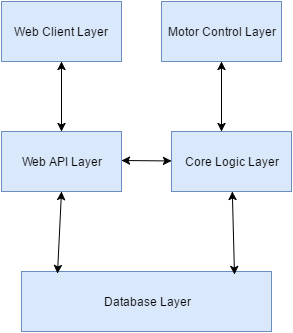
\includegraphics[width=0.60\textwidth]{images/layers}
 \caption{A simple architectural layer diagram}
\end{figure}

\subsection{Web API Description}
The Web API Layer serves data to the web client and any api callers through a http gateway. Access is controlled through an authentication engine which will only allow API calls from a registered client. Data is fetched by a data interface and transformed as required by the core program to be served to any requesting client. 

\subsection{Database Description}
The Database Layer is the primary store of all data in the application. It will keep a persistent store of configuration for the application so that the system can be restarted from a blank state without losing critical information such as the plants in the garden, the growth state of those plants, and actions made to those plants. The database layer will also compress data to maximize space efficiency. 

\subsection{Core Logic Description}
The Core Logic Layer acts as the central controller for the total system. Its most important job is to orchestrate a command pipeline to execute tasks on itself and the rest of the system. Secondarily, it also is responsible for generating commands for the motor control interface. Finally, it drives communication to the motor control unit based on instructions in the command pipeline. This communication is pushed through a serial interface via a G-Code executor routine. Most communication to other layers is accomplished through a restful html API. 

\subsection{Motor Control Description}
Motor Control Layer consists of Serial Command Interface, G-Code processor, I/O Handler, Stepper Controller, Sensor Controller. This layer is responsible to execute the processes in the command pipeline to control the motors. 

\subsection{Web Client Description}
The Web Client Layer displays system information to the user. It will consist of a JavaScript framework, static content, and a data service. 